\documentclass[tikz,border=3pt]{standalone}
\usetikzlibrary{arrows.meta,calc}
\begin{document}
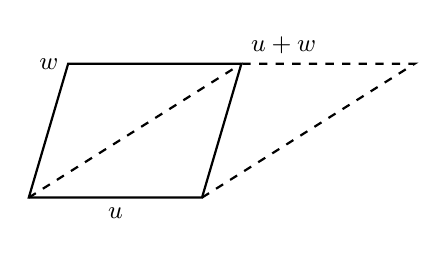
\begin{tikzpicture}[>=Latex, font=\small]
  \coordinate (O) at (0,0);
  \coordinate (U) at (2.2,0);
  \coordinate (W) at (0.5,1.7);
  \coordinate (UW) at ($(U)+(W)$);
  \coordinate (2UW) at ($(U)+(UW)$);

  \draw[thick, dashed] (U) -- (2UW) -- (UW);
  \draw[thick, dashed] (O) -- (UW);
  \draw[thick] (O) -- (U) -- (UW) -- (W) -- cycle;

  \node[left] at (W) {$w$};
  \node[above right] at (UW) {$u+w$};
  \node[below] at ($(O)!0.5!(U)$) {$u$};
\end{tikzpicture}
\end{document}
